% Options for packages loaded elsewhere
\PassOptionsToPackage{unicode}{hyperref}
\PassOptionsToPackage{hyphens}{url}
\PassOptionsToPackage{dvipsnames,svgnames,x11names}{xcolor}
%
\documentclass[
  letterpaper,
  DIV=11,
  numbers=noendperiod]{scrartcl}

\usepackage{amsmath,amssymb}
\usepackage{lmodern}
\usepackage{iftex}
\ifPDFTeX
  \usepackage[T1]{fontenc}
  \usepackage[utf8]{inputenc}
  \usepackage{textcomp} % provide euro and other symbols
\else % if luatex or xetex
  \usepackage{unicode-math}
  \defaultfontfeatures{Scale=MatchLowercase}
  \defaultfontfeatures[\rmfamily]{Ligatures=TeX,Scale=1}
\fi
% Use upquote if available, for straight quotes in verbatim environments
\IfFileExists{upquote.sty}{\usepackage{upquote}}{}
\IfFileExists{microtype.sty}{% use microtype if available
  \usepackage[]{microtype}
  \UseMicrotypeSet[protrusion]{basicmath} % disable protrusion for tt fonts
}{}
\makeatletter
\@ifundefined{KOMAClassName}{% if non-KOMA class
  \IfFileExists{parskip.sty}{%
    \usepackage{parskip}
  }{% else
    \setlength{\parindent}{0pt}
    \setlength{\parskip}{6pt plus 2pt minus 1pt}}
}{% if KOMA class
  \KOMAoptions{parskip=half}}
\makeatother
\usepackage{xcolor}
\setlength{\emergencystretch}{3em} % prevent overfull lines
\setcounter{secnumdepth}{5}
% Make \paragraph and \subparagraph free-standing
\ifx\paragraph\undefined\else
  \let\oldparagraph\paragraph
  \renewcommand{\paragraph}[1]{\oldparagraph{#1}\mbox{}}
\fi
\ifx\subparagraph\undefined\else
  \let\oldsubparagraph\subparagraph
  \renewcommand{\subparagraph}[1]{\oldsubparagraph{#1}\mbox{}}
\fi


\providecommand{\tightlist}{%
  \setlength{\itemsep}{0pt}\setlength{\parskip}{0pt}}\usepackage{longtable,booktabs,array}
\usepackage{calc} % for calculating minipage widths
% Correct order of tables after \paragraph or \subparagraph
\usepackage{etoolbox}
\makeatletter
\patchcmd\longtable{\par}{\if@noskipsec\mbox{}\fi\par}{}{}
\makeatother
% Allow footnotes in longtable head/foot
\IfFileExists{footnotehyper.sty}{\usepackage{footnotehyper}}{\usepackage{footnote}}
\makesavenoteenv{longtable}
\usepackage{graphicx}
\makeatletter
\def\maxwidth{\ifdim\Gin@nat@width>\linewidth\linewidth\else\Gin@nat@width\fi}
\def\maxheight{\ifdim\Gin@nat@height>\textheight\textheight\else\Gin@nat@height\fi}
\makeatother
% Scale images if necessary, so that they will not overflow the page
% margins by default, and it is still possible to overwrite the defaults
% using explicit options in \includegraphics[width, height, ...]{}
\setkeys{Gin}{width=\maxwidth,height=\maxheight,keepaspectratio}
% Set default figure placement to htbp
\makeatletter
\def\fps@figure{htbp}
\makeatother
\newlength{\cslhangindent}
\setlength{\cslhangindent}{1.5em}
\newlength{\csllabelwidth}
\setlength{\csllabelwidth}{3em}
\newlength{\cslentryspacingunit} % times entry-spacing
\setlength{\cslentryspacingunit}{\parskip}
\newenvironment{CSLReferences}[2] % #1 hanging-ident, #2 entry spacing
 {% don't indent paragraphs
  \setlength{\parindent}{0pt}
  % turn on hanging indent if param 1 is 1
  \ifodd #1
  \let\oldpar\par
  \def\par{\hangindent=\cslhangindent\oldpar}
  \fi
  % set entry spacing
  \setlength{\parskip}{#2\cslentryspacingunit}
 }%
 {}
\usepackage{calc}
\newcommand{\CSLBlock}[1]{#1\hfill\break}
\newcommand{\CSLLeftMargin}[1]{\parbox[t]{\csllabelwidth}{#1}}
\newcommand{\CSLRightInline}[1]{\parbox[t]{\linewidth - \csllabelwidth}{#1}\break}
\newcommand{\CSLIndent}[1]{\hspace{\cslhangindent}#1}

\KOMAoption{captions}{tableheading}
\makeatletter
\makeatother
\makeatletter
\makeatother
\makeatletter
\@ifpackageloaded{caption}{}{\usepackage{caption}}
\AtBeginDocument{%
\ifdefined\contentsname
  \renewcommand*\contentsname{Table of contents}
\else
  \newcommand\contentsname{Table of contents}
\fi
\ifdefined\listfigurename
  \renewcommand*\listfigurename{List of Figures}
\else
  \newcommand\listfigurename{List of Figures}
\fi
\ifdefined\listtablename
  \renewcommand*\listtablename{List of Tables}
\else
  \newcommand\listtablename{List of Tables}
\fi
\ifdefined\figurename
  \renewcommand*\figurename{Figure}
\else
  \newcommand\figurename{Figure}
\fi
\ifdefined\tablename
  \renewcommand*\tablename{Table}
\else
  \newcommand\tablename{Table}
\fi
}
\@ifpackageloaded{float}{}{\usepackage{float}}
\floatstyle{ruled}
\@ifundefined{c@chapter}{\newfloat{codelisting}{h}{lop}}{\newfloat{codelisting}{h}{lop}[chapter]}
\floatname{codelisting}{Listing}
\newcommand*\listoflistings{\listof{codelisting}{List of Listings}}
\makeatother
\makeatletter
\@ifpackageloaded{caption}{}{\usepackage{caption}}
\@ifpackageloaded{subcaption}{}{\usepackage{subcaption}}
\makeatother
\makeatletter
\@ifpackageloaded{tcolorbox}{}{\usepackage[many]{tcolorbox}}
\makeatother
\makeatletter
\@ifundefined{shadecolor}{\definecolor{shadecolor}{rgb}{.97, .97, .97}}
\makeatother
\makeatletter
\makeatother
\ifLuaTeX
  \usepackage{selnolig}  % disable illegal ligatures
\fi
\IfFileExists{bookmark.sty}{\usepackage{bookmark}}{\usepackage{hyperref}}
\IfFileExists{xurl.sty}{\usepackage{xurl}}{} % add URL line breaks if available
\urlstyle{same} % disable monospaced font for URLs
\hypersetup{
  pdftitle={On the Chicken \& Egg Problem in Transportation Electrification},
  pdfauthor={Jason Hawkins},
  colorlinks=true,
  linkcolor={blue},
  filecolor={Maroon},
  citecolor={Blue},
  urlcolor={Blue},
  pdfcreator={LaTeX via pandoc}}

\title{On the Chicken \& Egg Problem in Transportation Electrification}
\author{Jason Hawkins}
\date{}

\begin{document}
\maketitle
\ifdefined\Shaded\renewenvironment{Shaded}{\begin{tcolorbox}[interior hidden, frame hidden, enhanced, boxrule=0pt, borderline west={3pt}{0pt}{shadecolor}, sharp corners, breakable]}{\end{tcolorbox}}\fi

\hypertarget{introduction}{%
\section{Introduction}\label{introduction}}

Vehicle electrification is widely regarded as a critical tool for
climate change mitigation in the transportation sector (Musti and
Kockelman 2011). While the United States is seeing an increasing share
of electric sales, the pace of adoption remains well below the necessary
level to mitigate climate change impacts. One barrier to widespread
adoption is the lack of charging infrastructure (Sullivan and Taylor
2021).

\hypertarget{the-electric-vehicle-and-charging-station-problem}{%
\section{The Electric Vehicle and Charging Station
Problem}\label{the-electric-vehicle-and-charging-station-problem}}

Electric vehicle ownership is often referenced as exhibiting a ``chicken
and egg'' behavior arising from the supply and demand relationship.
Individual demand for electric vehicles is influenced by the available
supply of charging points. Consumers are unwilling to purchase vehicles
due to range anxiety and a perceived lack of charging stations.
Suppliers are not incentivized to provide charging stations unless there
is sufficient demand to warrant their cost. There is a clear role for
public policy in such situations. The government deems electric vehicles
as a solution to a public ill (i.e., climate change) and can incentivize
either suppliers by providing installation subsidies or consumers by
installing charging stations. While the problem has been recognized in
the literature (Melliger, Vliet, and Liimatainen 2018), empirical
analysis is minimal.

An important consideration to the analysis is how electric mobility
system may differ from one based on fossil fuels. In the conventional
private mobility model, the individual owns the vehicle and purchases
fuel from centralized and privately owned refueling stations. In
contrast, electric vehicles may be charged in the home using previously
existing infrastructure. The presence of charging points in the home
begs the questions 1) if (or to what extent) out-of-home charging
stations are required for travel? and 2) to what extent is range anxiety
a perception versus a reality?

According to the Bureau of Transportation Statistics, 98\% of trips made
in the US are less than 50 miles (Vehicle Technology Office 2022). Given
that most battery-electric vehicles (BEVs) have a range greater than 200
miles (Elfalan 2021), it is feasible to make most trips on a single
charge. However, long-distance trips (over 50 miles) comprise 30\% of
total vehicle-miles traveled (VMT) (Aultman-Hall 2018). There is clearly
a need for out-of-home charging stations to accommodate these trips.
Even if most trips can be accommodated by in-home charging, the vehicle
purchase decision will be influenced by consideration of these longer
trips that require charging stations (Silvia and Krause 2016).
Additionally, Wolbertus et al. (Wolbertus et al. 2018) find that there
is still a demand for charging stations in places where public daytime
charging is the only option, such as at the workplace.

\hypertarget{data-sources}{%
\section{Data Sources}\label{data-sources}}

We use a combination of open-source and purchased data in our analysis.
The two key input datasets are charging station locations provided by
the Alternative Fuel Data Center (AFDC) and electric vehicle
registrations provided by Experian Inc.~The vehicle registration dataset
comprises a 10-year panel at 2-year increments (i.e., 2012, 2014, 2016,
2018, 2020). Total vehicle registrations are recorded by county for the
United States.

This initial analysis is based on the charging station data and EV sales
by state for the period 2013 to 2020 as the county-level registrations
were not made available in time for publication. EV sales and market
share data is provided by EVAdoption, and state population data by the
U.S. Census Bureau.

\begin{verbatim}
C:\Users\jhawkins17\AppData\Local\Temp\ipykernel_15120\2346844971.py:2: DtypeWarning: Columns (6,20) have mixed types. Specify dtype option on import or set low_memory=False.
  df_ch_stn = pd.read_csv("../Data/Transport/alt_fuel_stations_w_county.csv")
\end{verbatim}

\begin{verbatim}
df_ch_stn all 53684
df_ch_stn no private 49852
df_ch_stn (after removing nan open year 49846
\end{verbatim}

TO DO: - plot total vehicles and total charging stations per person -
create county-specific Granger causality statistics - Input demographic
data by county - create generalized propensity scores - create
regression inputs - run regressions - write literature review - write
results and discussion - get casey's stuff working in the paper - write
up methods

\hypertarget{methods}{%
\section{Methods}\label{methods}}

\hypertarget{results}{%
\section{Results}\label{results}}

\begin{figure}

\begin{minipage}[t]{\linewidth}

{\centering 

\raisebox{-\height}{

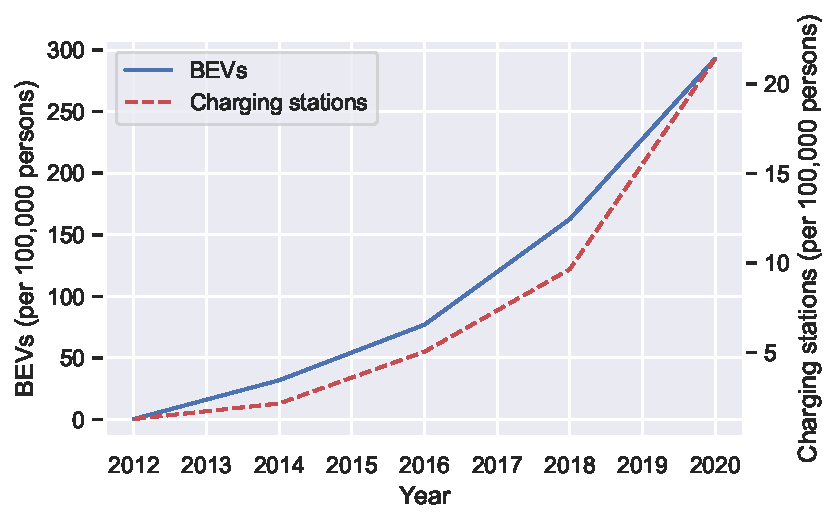
\includegraphics{TRB_2023_files/figure-pdf/cell-4-output-1.pdf}

}

\caption{US BEV Registrations and Charging Stations}

}

\end{minipage}%

\end{figure}

\texttt{\{\#\ \{python\}\ \#\ \#\#\ Number\ of\ Charging\ stations\ per\ county\ \#\ ax\ =\ gplt.choropleth(\ \#\ \ \ final{[}final{[}\textquotesingle{}STATEFP\textquotesingle{}{]}\ ==\ 6{]},\ \#\ \ \ hue\ =\ "Charging\ Stations",\ \#\ \ \ edgecolor=\textquotesingle{}darkgrey\textquotesingle{},\ \#\ \ \ linewidth=.5,\ \#\ \ \ cmap="viridis",\ \#\ \ \ legend=True,\ \#\ \ \ projection=gcrs.AlbersEqualArea(),\ \#\ \ \ figsize\ =\ (16,16),\ \#\ \ \ zorder\ =\ 1\ \#\ )\ \#\ \ \#\ gplt.pointplot(\ \#\ \ \ station\_points{[}station\_points{[}\textquotesingle{}STATEFP\textquotesingle{}{]}\ ==\ 6{]},\ \#\ \ \ projection=gcrs.AlbersEqualArea(),\ \#\ \ \ ax\ =\ ax,\ \#\ \ \ zorder\ =\ 2,\ \#\ \ \ s\ =\ .4\ \#\ )}

\hypertarget{discussion}{%
\section{Discussion}\label{discussion}}

\hypertarget{conclusions}{%
\section{Conclusions}\label{conclusions}}

The results presented herein are preliminary and do not consider a key
dataset -- vehicle registrations. We will expand our analysis to a more
robust inferential study in the coming months. Our causal question is
what effect public charging stations have on electric vehicle
registrations at the county-level. The treatment variable is continuous
over the study period. We propose three causal identification
approaches. The first approach is a difference-in-differences approach
that is identified off state-level investments in charging stations by
year. The second approach is generalized propensity score matching using
federal election results, state-level greenhouse gas (GHG) emissions
factors, and demographic characteristics (e.g., racial composition,
median income, and population density) as inputs to the propensity
score.

The final causal inference approach, Granger causality, differs in that
it focuses on the temporal phasing of charging station installations and
PEV registration, whereas the other two approaches rely on Rubin's
potential outcome assumption (Reich et al. 2021). Granger causality
relies on the assumption that past treatment knowledge reduces
predictive uncertainty. It is a form of time series causal inference
that would fit the current context well.

\hypertarget{section}{%
\section*{}\label{section}}
\addcontentsline{toc}{section}{}

\hypertarget{refs}{}
\begin{CSLReferences}{1}{0}
\leavevmode\vadjust pre{\hypertarget{ref-aultman-hall2018}{}}%
Aultman-Hall, Lisa. 2018. {``Incorporating Long-Distance Travel into
Transportation Planning in the United States.''}
\url{https://escholarship.org/uc/item/0ft8b3b5}.

\leavevmode\vadjust pre{\hypertarget{ref-elfalan2021}{}}%
Elfalan, Jonathan. 2021. {``Electric Car Range and Consumption.''}
\url{https://www.edmunds.com/car-news/electric-car-range-and-consumption-epa-vs-edmunds.html}.

\leavevmode\vadjust pre{\hypertarget{ref-melliger2018}{}}%
Melliger, Marc A., Oscar P. R. van Vliet, and Heikki Liimatainen. 2018.
{``Anxiety Vs Reality {\textendash} Sufficiency of Battery Electric
Vehicle Range in Switzerland and Finland.''} \emph{Transportation
Research Part D: Transport and Environment} 65 (December): 101--15.
\url{https://doi.org/10.1016/J.TRD.2018.08.011}.

\leavevmode\vadjust pre{\hypertarget{ref-musti2011}{}}%
Musti, Sashank, and Kara M. Kockelman. 2011. {``Evolution of the
Household Vehicle Fleet: Anticipating Fleet Composition, PHEV Adoption
and GHG Emissions in Austin, Texas.''} \emph{Transportation Research
Part A: Policy and Practice} 45 (8): 707--20.
\url{https://doi.org/10.1016/J.TRA.2011.04.011}.

\leavevmode\vadjust pre{\hypertarget{ref-reich2021}{}}%
Reich, Brian J., Shu Yang, Yawen Guan, Andrew B. Giffin, Matthew J.
Miller, and Ana Rappold. 2021. {``A Review of Spatial Causal Inference
Methods for Environmental and Epidemiological Applications.''}
\emph{International Statistical Review} 89 (3): 605--34.
\url{https://doi.org/10.1111/insr.12452}.

\leavevmode\vadjust pre{\hypertarget{ref-silvia2016}{}}%
Silvia, Chris, and Rachel M. Krause. 2016. {``Assessing the Impact of
Policy Interventions on the Adoption of Plug-in Electric Vehicles: An
Agent-Based Model.''} \emph{Energy Policy} 96 (September): 105--18.
\url{https://doi.org/10.1016/J.ENPOL.2016.05.039}.

\leavevmode\vadjust pre{\hypertarget{ref-sullivan2021}{}}%
Sullivan, Brian, and Harriet Taylor. 2021. {``The u.s. EV Charging
Network Isn't Ready for Your Family Road Trip, Let Alone the Expected
Wave of New Cars.''}
\url{https://www.cnbc.com/2021/08/24/cnbc-road-test-the-us-ev-charging-network-isnt-ready-for-your-family-road-trip-let-alone-the-expected-wave-of-new-cars.html}.

\leavevmode\vadjust pre{\hypertarget{ref-vehicletechnologyoffice2022}{}}%
Vehicle Technology Office. 2022. {``More Than Half of All Daily Trips
Were Less Than Three Miles in 2021.''}
\url{https://www.energy.gov/eere/vehicles/articles/fotw-1230-march-21-2022-more-half-all-daily-trips-were-less-three-miles-2021}.

\leavevmode\vadjust pre{\hypertarget{ref-wolbertus2018}{}}%
Wolbertus, Rick, Maarten Kroesen, Robert van den Hoed, and Caspar G.
Chorus. 2018. {``Policy Effects on Charging Behaviour of Electric
Vehicle Owners and on Purchase Intentions of Prospective Owners: Natural
and Stated Choice Experiments.''} \emph{Transportation Research Part D:
Transport and Environment} 62 (July): 283--97.
\url{https://doi.org/10.1016/j.trd.2018.03.012}.

\end{CSLReferences}



\end{document}
